\documentclass[en,license=none]{../../../eplsummary}

\usepackage{float}

\graphicspath{{img/}}

\hypertitle{Computer networks}{5}{INGI}{1341}
{Gilles Peiffer}
{Olivier Bonaventure}

\section{Connecting two hosts}

The first step when building a network,
even a worldwide network such as the Internet,
is to connect two hosts together.
In order for two hosts to exchange information,
they need to be linked by some kind of physical medium.
Various types of media have been used for this purpose:
\begin{itemize}
	\item \emph{Electrical cable}.
	Different types of cables are suitable for transmitting information:
	\begin{itemize}
		\item twisted pairs,
		which are used in the telephone network
		and in enterprise networks;
		\item coaxial cables,
		which are used in cable TV networks,
		but not in enterprise networks anymore.
	\end{itemize}
	Some technologies operate over the classical electrical cable.
	\item \emph{Optical fiber}.
	Optical fibers are used in networks
	when the distance between the devices is larger than one kilometer.
	There are two main types of optical fibers:
	\begin{itemize}
		\item multimode, which uses a LED to send signals
		over distances greater than several tens of kilometers;
		\item monomode, which uses a laser to send signals
		over distances of a few kilometers.
	\end{itemize}
	Both types can use repeaters to regenerate the signal
	and send it over another fiber.
	\item \emph{Wireless}.
	With this technology,
	a radio signal is used to encode the exchanged information.
	Modulation techniques are used
	to send information over a wireless channel.
	Some wireless networks use a laser
	that sends light pulses to a detector
	instead of a radio signal.
	These optical techniques allow to create point-to-point links,
	while radio based techniques can be used
	to build networks containing devices
	spread over a small geographical area.
\end{itemize}

\subsection{The physical layer}

The physical media explained previously can be used to exchange information,
once this information has been converted into a suitable electrical signal.
We will focus on the transmission of bits, i.e. either $0$ or $1$.

\begin{mydef}[Bit rate]
	In computer networks, the bit rate of the physical layer
	is always expressed in bits per second.
	This is in contrast with memory specifications
	which are usually expressed in bytes
	(one byte is equal to eight bits).
\end{mydef}

\subsubsection{Time-sequence diagram}

A physical transmission scheme
(interactions between communicating hosts)
can be described by using a \emph{time-sequence diagram}.
By convention, the sender is represented on the left,
and the receiver is on the right.
The middle of the diagram represents the electrical link.
Time flows from top to bottom.
To represent the transmission of a single bit,
three arrows are needed.
\begin{enumerate}
	\item The sender receives a request to transmit one bit of information.
	A \emph{primitive} is used to represent this request,
	sort of like a procedure call.
	The bit being transmitted is the only parameter.
	In the example in \figuref{timeseqdiag},
	the primitive is named \texttt{DATA.request}.
	\item The dashed arrow indicates the signal's propagation time
	between the two hosts.
	Once the signal is received,
	it's interpreted and converted into a bit.
	\item The bit is delivered as a \texttt{DATA.indication} primitive.
\end{enumerate}

\begin{figure}[H]
	\centering
	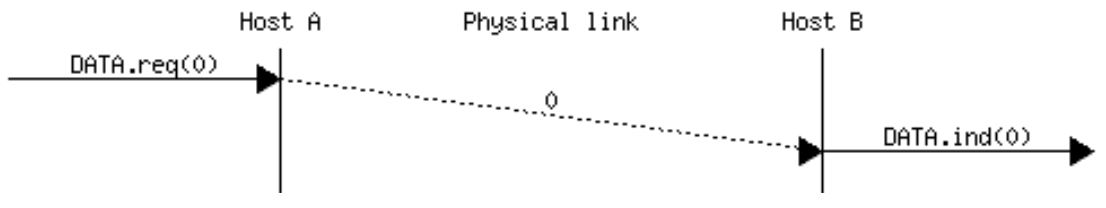
\includegraphics[width=\textwidth]{timeseqdiag.png}
	\caption{A simple time-sequence diagram.}
	\label{fig:timeseqdiag}
\end{figure}

One of the problems of such a transmission scheme
is that electromagnetic interference can switch bits
while they're being transmitted
(i.e. a $0$ bit is sent but a $1$ bit is received).

With the above transmission scheme,
a bit is transmitted by setting the voltage on the electrical cable
to a specific value during some period of time.
One source of errors can be the difference in measured voltage
between the sender and the receiver.
Another reason could be that the two clocks do not operate
at exactly the same frequency.
Small differences in clock frequency imply
that bits can ``disappear'' or ``appear''
during their transmission on an electrical cable
(as in \figuref{lostbitdiag}).

\begin{figure}[H]
	\centering
	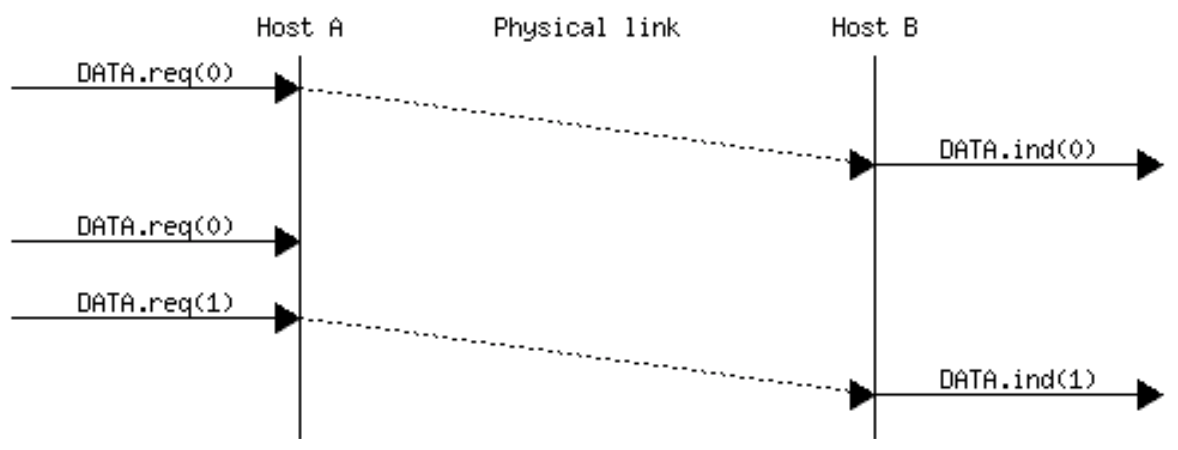
\includegraphics[width=\textwidth]{lostbitdiag.png}
	\caption{Bits can ``disappear'' due to mismatched clock frequencies.}
	\label{fig:lostbitdiag}
\end{figure}

Due to these possible sources of error,
it's important to remember that the physical layer service may
\begin{itemize}
	\item \textbf{change} the value of a bit being transmitted,
	\item \textbf{deliver more (or less)} bits to the receiver
	than the bits sent by the sender.
\end{itemize}

\paragraph{Manchester encoding} Other types of encodings have been defined
to transmit information over an electrical cable.
All physical layers are able to send and receive physical symbols
that represent the values $0$ and $1$.
However, for various reasons that are outside the scope of this chapter,
several physical layers exchange other physical symbols as well.
The Manchester encoding is an encoding scheme
in which time is divided into fixed-length periods.
Each period is divided into two halves
during which different voltage levels (high or low) can be applied.
The four possible combinations make for four possible characters,
as shown in \figuref{manchester_encoding}.

\begin{figure}[H]
	\centering
	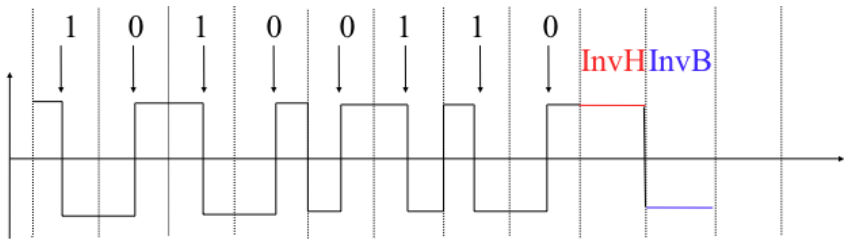
\includegraphics[width=\textwidth]{manchester_encoding.png}
	\caption{Visualisation of the Manchester encoding.
	$0$ and $1$ are regular bits,
	the InvH and InvB symbols can be used as markers
	for the beginning or end of frames.}
	\label{fig:manchester_encoding}
\end{figure}

\subsection{The datalink layer}

The physical layer is the name given
to all the functions related to the physical transmission of information.
It allows two or more entities to exchange bits
if they are connected to the same medium.
Computer networks use different layers,
where each layer provides a service that is built above the underlying layer,
and is close to the needs of the applications.
The datalink layer builds upon the service provided by the physical layer.
\bigbreak
\subsubsection{Framing}
\begin{mydef}[Frame]
	In many networks, the fundamental unit of of information
	exchanged between two hosts is called a \emph{frame}.
	A \emph{frame} is a sequence of bits
	that has a particular syntax or structure.
\end{mydef}
\begin{myrem}[Bit rate and bandwidth]
	Bit rate and bandwidth are often used
	to characterize the transmission capacity of the physical service.
	Bandwidth is defined as ``a range of radio frequencies
	which is occupied by a modulated carrier wave,
	which is assigned to a service,
	or over which a device can operate''.
	By extension, bandwidth is also used
	to represent the capacity of a communication system in bits per second.
\end{myrem}
Since the physical layer is not perfect,
transmitting and receiving frames
is not as simple as just defining a way to encode frames into bits,
or make out frames from bits.
A generic solution exists that works on any physical layer: \emph{stuffing}.
To enable a receiver to easily delineate the frame boundaries,
special bit strings serve as frame boundary markers
and encode the frames so that these special bit strings
do not appear inside the frames.
There are two variants of \emph{stuffing}:
\begin{itemize}
	\item \emph{Bit stuffing}.
	Bit stuffing reserves the $01111110$ bit string
	as the frame boundary marker
	and ensures there will never be six consecutive $1$ symbols
	transmitted by the physical layer inside a frame.
	It works as follows:
	\begin{enumerate}
		\item The sender transmits the marker, i.e. $01111110$.
		\item The sender sends all the bits of the frame
		and inserts an additional bit set to $0$
		after each sequence of five consecutive $1$ bits.
		\item The sender transmits the marker again,
		marking the end of the frame.
		\item The receiver detects the beginning of a frame
		thanks to the marker.
		\item The receiver processes the received bits,
		and if it counts five consecutive bits set to $1$,
		followed by a $0$ bit,
		that last bit is discarded.
		\item Once the receiver detects the marker again,
		it knows the frame has been received entirely.
	\end{enumerate}
	Bit stuffing increases the number of bits
	required to transmit the frame,
	with the worst case being
	a long sequence of bits set to $1$ inside the frame.
	Note that bit stuffing is vulnerable to transmission errors.
	If such an error happens,
	the frame (and possible the next)
	will not correctly be decoded by the receiver,
	but it will be able to resynchronize itself at the next valid marker.
	\item \emph{Character stuffing}.
	Character stuffing techniques
	use control characters in the ASCII table
	as markers to delineate frame boundaries.
	The following markers are often used:
	DLE STX to mark the beginning and DLE ETX to mark the end\footnote{DLE ($0010000$ b) for ``Data Link Escape'',
	STX ($0000010$ b) for ``Start of Text''
	and ETX ($0000011$ b) for ``End of Text''.}.
	When transmitting a frame,
	the sender adds a DLE character after each transmitted DLE character.
	This ensures that none of the markers
	can appear inside the transmitted frame.
	The receiver detects this
	and removes the second DLE when it receives two consecutive ones.
	Just like bit stuffing,
	character stuffing increases the length of the transmitted frames.
	The worst frame for character stuffing
	is a frame containing many DLE characters.
	Again, two frames can potentially be lost
	when a transmission error occurs,
	but the receiver will be able to resynchronize itself
	with the next correctly received markers.
\end{itemize}
While bit stuffing is easily implemented in hardware,
it is difficult to implement in software
given the complexity of performing bit manipulations in software.
Software implementations prefer to use character stuffing instead.

Both of these techniques allow to recover frames from a stream of bits or bytes.
The framing mechanism provides a richer service than the physical layer.
It can also be represented using the DATA.req and DATA.ind primitives,
as illustrated in \figuref{stuffing_diag}.

\begin{figure}[H]
	\centering
	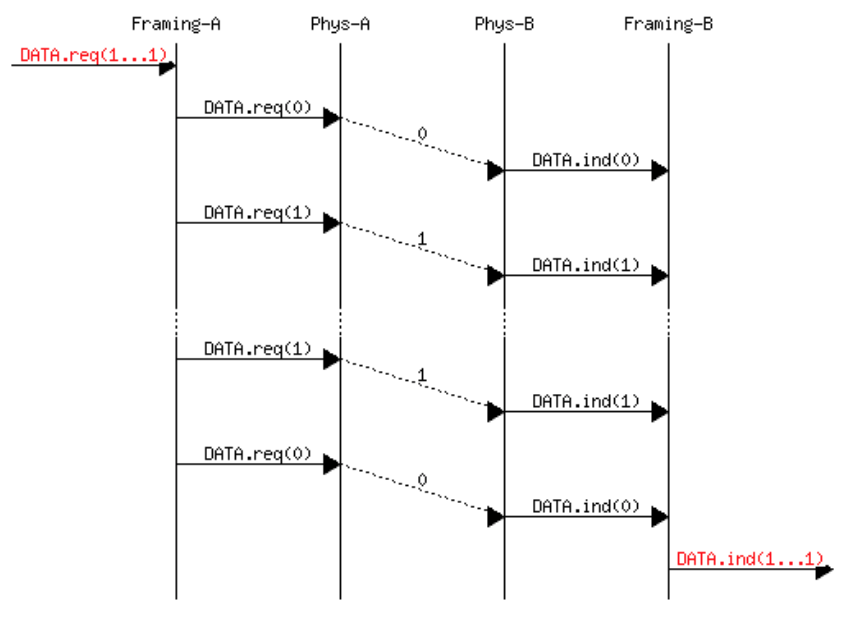
\includegraphics[width=0.4\textwidth]{stuffing_diag.png}
	\caption{Time-sequence diagram of framing,
	assuming hypothetical frames containing four useful bits
	and one bit of framing.}
	\label{fig:stuffing_diag}
\end{figure}

\subsubsection{Recovering from transmission errors}
\end{document}
